\documentclass[aspectratio=169, 11pt]{beamer}

% ===================== PACKAGES =====================
\usepackage{lmodern}
\usepackage[T1]{fontenc}
\usepackage[utf8]{inputenc}
\usepackage{graphicx}
\usepackage{booktabs}
\usepackage{xcolor}
\usepackage{amsmath}
\usepackage{tabularx}
\usepackage{array}
\usepackage{colortbl}

% ===================== COLORS (matching report) =====================
\definecolor{inertiapurple}{HTML}{6B3FA0}
\definecolor{inertiablue}{HTML}{1A3D7C}
\definecolor{lightpurple}{HTML}{EFEAF5}
\definecolor{rulegrey}{HTML}{D0D0D0}

% ===================== BEAMER THEME =====================
\usetheme{default}
\usecolortheme{default}
\setbeamersize{text margin left=14mm, text margin right=14mm}

% Kill default clutter
\setbeamertemplate{navigation symbols}{}
\setbeamertemplate{headline}{}

% Frame title: purple, bold, rule below
\setbeamercolor{frametitle}{fg=inertiapurple, bg=white}
\setbeamerfont{frametitle}{series=\bfseries, size=\Large}
\setbeamertemplate{frametitle}{%
  \vspace{10pt}
  \hspace{-2pt}\insertframetitle
  \vspace{-8pt}\\[2pt]
  {\color{inertiapurple}\rule{\textwidth}{0.4pt}}%
}

% Title colors (for \title, \author, etc.)
\setbeamercolor{title}{fg=inertiapurple}
\setbeamercolor{subtitle}{fg=black}
\setbeamercolor{author}{fg=black}
\setbeamercolor{institute}{fg=black}
\setbeamercolor{structure}{fg=inertiapurple}
\setbeamercolor{alerted text}{fg=inertiapurple}

% Minimal footer: purple rule + page N of N on the right
\setbeamertemplate{footline}{%
  \leavevmode%
  \hbox{\begin{beamercolorbox}[wd=\paperwidth, ht=3ex, dp=1.5ex, leftskip=14mm, rightskip=14mm]{footerline}%
  {\color{rulegrey}\rule{\textwidth}{0.3pt}}\\
  \hspace*{0pt}\hfill{\tiny\color{gray}\insertframenumber\,/\,\inserttotalframenumber}%
  \end{beamercolorbox}}%
}

% Bullet styling
\setbeamertemplate{itemize item}{\color{inertiapurple}\footnotesize$\blacksquare$}
\setbeamertemplate{itemize subitem}{\color{inertiablue}\scriptsize$\bullet$}
\setbeamerfont{itemize/enumerate body}{size=\normalsize}

% Caption styling
\setbeamercolor{caption name}{fg=inertiablue}

% ===================== MACROS =====================
\newcommand{\fundname}{\textsc{Inertia}}
\newcommand{\emphp}[1]{{\color{inertiapurple}\textbf{#1}}}
\newcommand{\emphb}[1]{{\color{inertiablue}\textbf{#1}}}

% ===================== DOCUMENT =====================
\begin{document}

% =========================================================
% SLIDE 1: TITLE
% =========================================================
\begin{frame}[plain]
  \vspace{0.8cm}
  \begin{center}
    {\Huge\bfseries\color{inertiapurple} Inertia}\\[10pt]
    {\large\itshape A Conditional Timing Strategy for the Momentum Factor}\\[24pt]
    {\color{inertiapurple}\rule{0.4\textwidth}{0.5pt}}\\[20pt]
    {\large Will Wu \,\textbullet\, Kathy Yang}\\[8pt]
    {\normalsize UG54 Data Driven Investing\, \textbullet\, Spring 2026}\\[4pt]
    {\small\color{inertiablue} Topic dimensions: Timing Strategies \;\textbullet\; Factor Investing \;\textbullet\; Machine Learning}\\[36pt]
    \begin{minipage}{0.75\textwidth}
      \centering
      {\itshape Sharpe 0.80 beats Daniel and Moskowitz's 0.74 out of sample\\ at the 5 percent significance level.}
    \end{minipage}
  \end{center}
\end{frame}

% =========================================================
% SLIDE 2: THE PITCH IN ONE NUMBER (hero chart)
% =========================================================
\begin{frame}{The pitch in one number}
  \vspace{-4pt}
  \begin{center}
    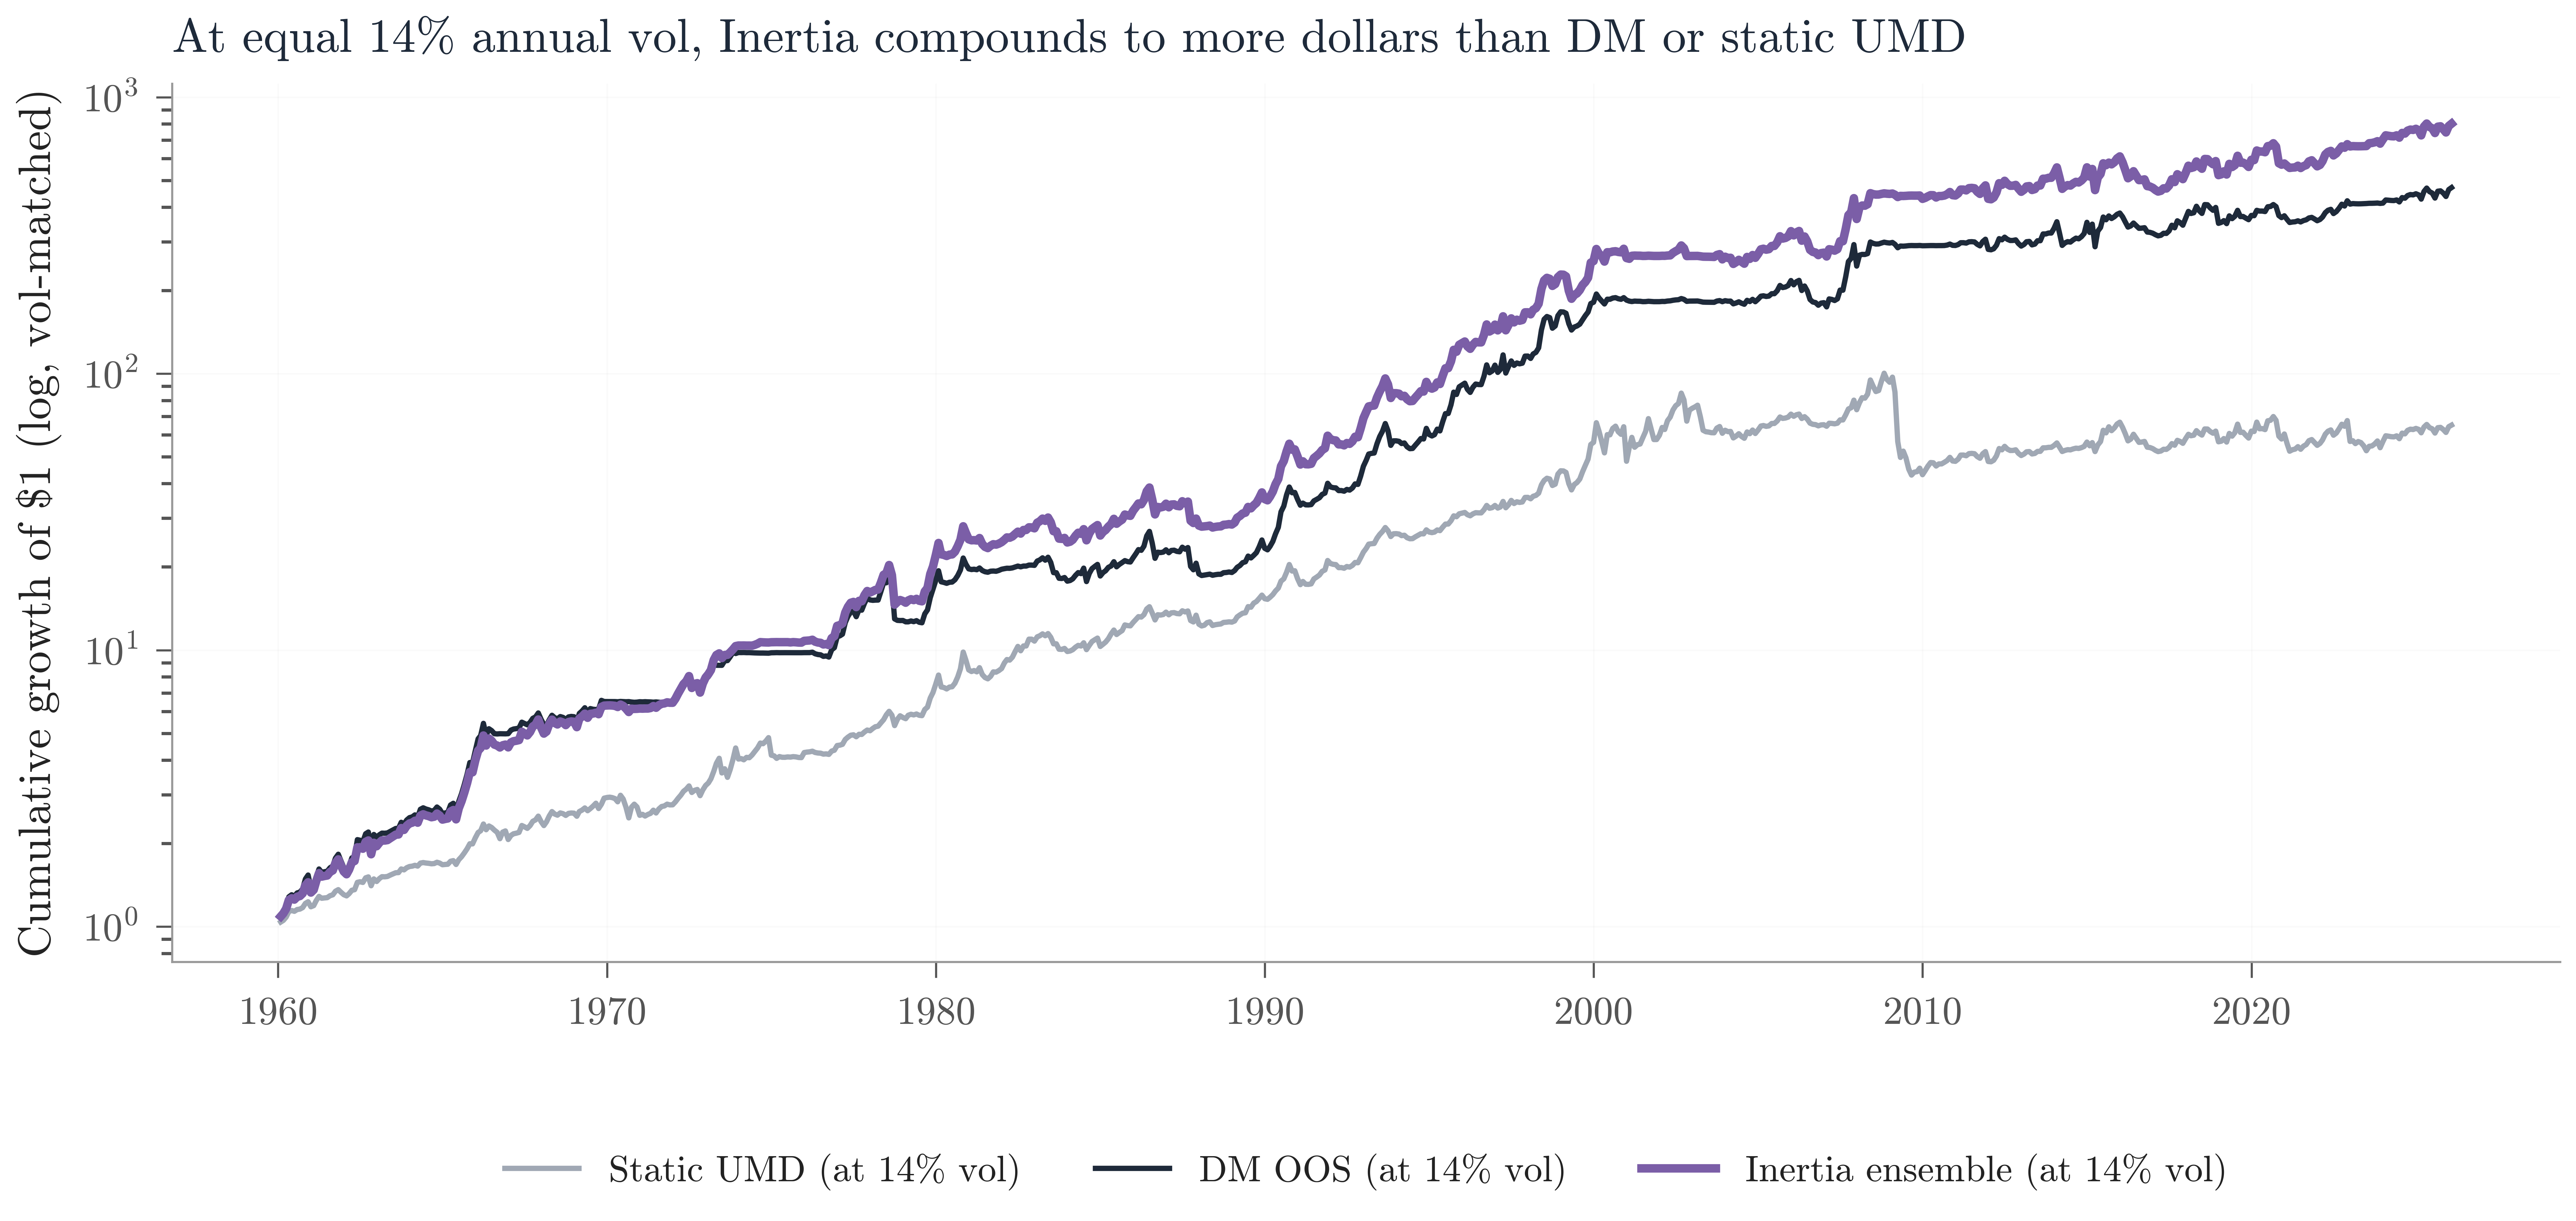
\includegraphics[width=0.95\textwidth]{figures/21_inertia_volmatched_cumret.png}
  \end{center}
  \vspace{-8pt}
  \begin{center}
  \small At equal 14 percent annualized volatility since 1960:
  \ static UMD $\to$ \$65,
  \ DM benchmark $\to$ \$471,
  \ \emphp{Inertia $\to$ \$802} per dollar invested.
  \end{center}
\end{frame}

% =========================================================
% SLIDE 3: PERFORMANCE AT A GLANCE
% =========================================================
\begin{frame}{Performance at a glance}
  \vspace{18pt}
  \begin{center}
  \small
  \begin{tabular}{l r r r r r}
    \toprule
     & \textbf{Mean} & \textbf{Vol} & \textbf{Sharpe} & \textbf{Alpha} & \textbf{Max DD} \\
    \midrule
    Static UMD    & 7.5\%  & 14.2\% & 0.53 & n/a    & $-58$\% \\
    DM benchmark  & 10.5\% & 14.2\% & 0.74 & 5.6\%  & $-34$\% \\
    \rowcolor{lightpurple}
    \textbf{\fundname}     & \textbf{8.5\%} & \textbf{10.7\%} & \textbf{0.80} & \textbf{4.0\%} & $\mathbf{-22}$\textbf{\%} \\
    \bottomrule
  \end{tabular}
  \end{center}
  \vspace{16pt}
  \begin{itemize}
    \item \emphb{Same Sharpe as DM at three-quarters the volatility}
    \item Max drawdown nearly one-third lower than DM, less than half of static
    \item Alpha of 4.0 percent annualized against Fama-French five-factor plus UMD ($t = 2.63$)
  \end{itemize}
  \vspace{4pt}
  {\footnotesize\color{gray} Out-of-sample 1960 through 2026, 793 months, net of 20 basis point one-way costs.}
\end{frame}

% =========================================================
% SLIDE 4: MOMENTUM IS RELIABLE BUT FRAGILE
% =========================================================
\begin{frame}{Momentum is reliable, but fragile}
  \vspace{4pt}
  \begin{columns}[T]
    \begin{column}{0.50\textwidth}
      
\includegraphics[width=\textwidth]{figures/01_umd_cumret_log.png}
    \end{column}
    \begin{column}{0.50\textwidth}
      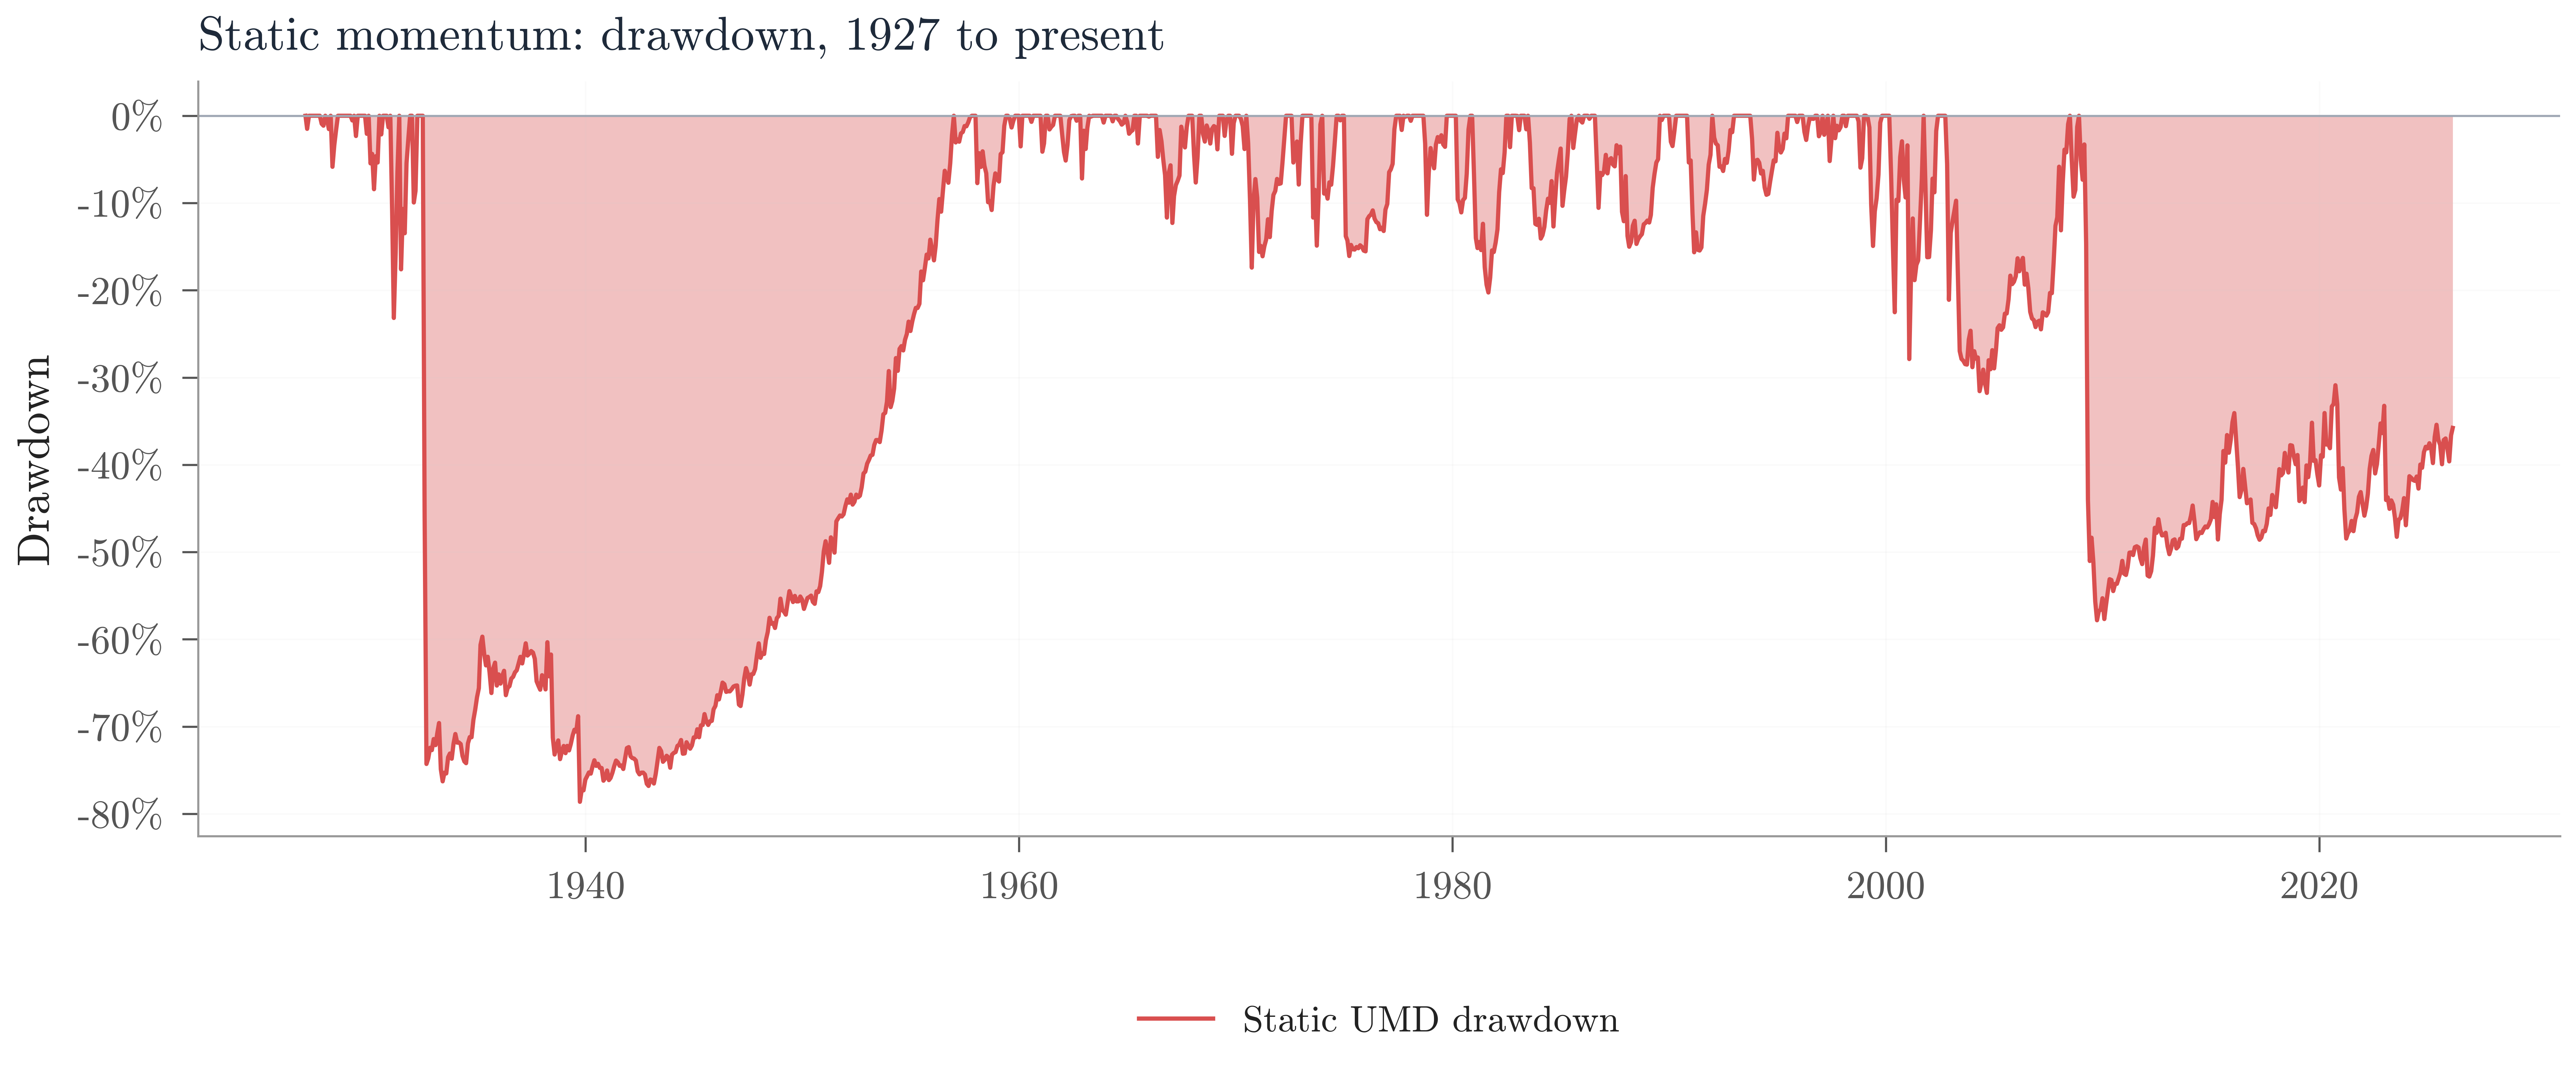
\includegraphics[width=\textwidth]{figures/02_umd_drawdown.png}
    \end{column}
  \end{columns}
  \vspace{10pt}
  \begin{itemize}
    \item Long-run Sharpe 0.53 since 1960; 7.5 percent annualized excess return at 14.2 percent volatility
    \item \emphp{But}: skew $-1.3$, excess kurtosis 10.0, three drawdowns exceeding 40 percent, peak of 58 percent
    \item Crashes are \emphb{structural}, not random: short leg concentrates in high-beta distressed names that rebound violently
  \end{itemize}
\end{frame}

% =========================================================
% SLIDE 5: DANIEL AND MOSKOWITZ (2015) BENCHMARK
% =========================================================
\begin{frame}{Academic benchmark: Daniel and Moskowitz (2015)}
  \vspace{6pt}
  \textbf{Predictive regression.} Conditional mean and variance of UMD are jointly forecastable from a 24-month bear-market indicator and trailing UMD realized variance:
  \begin{equation*}
    r^{UMD}_{t+1} \;=\; \alpha \;+\; \beta_1 I^{B}_t \;+\; \beta_2 (I^{B}_t \cdot \sigma^2_t) \;+\; \beta_3\, \sigma^2_t \;+\; \varepsilon_{t+1},
    \qquad \beta_2 < 0.
  \end{equation*}
  \vspace{2pt}
  \textbf{Dynamic mean-variance weight} (from the capital allocation unit):
  \begin{equation*}
    w^{DM}_t \;=\; c \cdot \frac{\widehat{E}_t[r^{UMD}_{t+1}]}{\widehat{\mathrm{Var}}_t[r^{UMD}_{t+1}]}
  \end{equation*}
  \vspace{6pt}
  \begin{itemize}
    \item OOS discipline: expanding window, annual refits, first OOS month January 1960
    \item \emphp{Sharpe 0.74}, 95\% CI $[0.47,\,0.97]$, max drawdown $-34$ percent
    \item This is the bar we must clear
  \end{itemize}
\end{frame}

% =========================================================
% SLIDE 6: APPROACH A (RIDGE)
% =========================================================
\begin{frame}{Approach A: Ridge regression, expanded linear}
  \vspace{6pt}
  \begin{itemize}
    \item \textbf{Idea:} keep DM's framework, expand the feature set
    \item DM originals $+$ market realized vol, market drawdown, UMD drawdown, lagged market returns (8 features)
    \item \textbf{Ridge} with 5-fold cross-validated L2 penalty, features standardized per window
  \end{itemize}
  \vspace{16pt}
  \begin{center}
  \begin{tabular}{l c c c}
    \toprule
     & \textbf{Sharpe} & \textbf{95\% CI} & \textbf{$\Delta$ vs DM} \\
    \midrule
    A (Ridge) & 0.69 & $[0.41,\,0.92]$ & $-0.05$ \\
    \bottomrule
  \end{tabular}
  \end{center}
  \vspace{14pt}
  \emphb{Honest finding:} L2 shrinkage attenuates DM's critical bear-times-variance interaction.  Additional linear features do not compensate.
\end{frame}

% =========================================================
% SLIDE 7: APPROACH B (CRASH SHIELD)
% =========================================================
\begin{frame}{Approach B: Gradient-boosted crash shield}
  \begin{itemize}
    \item \textbf{Reframe} as classification: label crash when $r^{UMD}_{t+1} < q_{10}$ (training set)
    \item Gradient-boosted trees on the same 8 features; binary shield rule:
    \[
      w^{B}_t = \begin{cases} 1 & \text{if } \hat{p}^{\text{crash}}_t < 0.05 \\ 0 & \text{otherwise} \end{cases}
    \]
    \textit{Threshold 0.05 is half the training baseline rate, chosen a priori.}
  \end{itemize}
  \vspace{-4pt}
  \begin{center}
    
\includegraphics[width=0.85\textwidth]{figures/13_approach_b_pcrash_timeseries.png}
  \end{center}
  \vspace{-2pt}
  \footnotesize Sharpe \textbf{0.63} at vol \textbf{8.2 percent}, max drawdown \textbf{$-24$ percent}, \emphp{positive skew $+0.43$} (only strategy with right-tail distribution).
\end{frame}

% =========================================================
% SLIDE 8: APPROACH C (HMM)
% =========================================================
\begin{frame}{Approach C: Unsupervised 2-state HMM}
  \begin{itemize}
    \item \textbf{No supervised labels.} Fit a 2-state Gaussian HMM on three observables: market return, market vol, UMD vol
    \item Forward algorithm gives filtered $P(\text{normal}_t \mid \text{obs}_{1..t})$ with no look-ahead
    \item \textbf{Weight} = $P(\text{normal}_t)$, continuous in $[0, 1]$, no threshold to tune
  \end{itemize}
  \vspace{-4pt}
  \begin{center}
    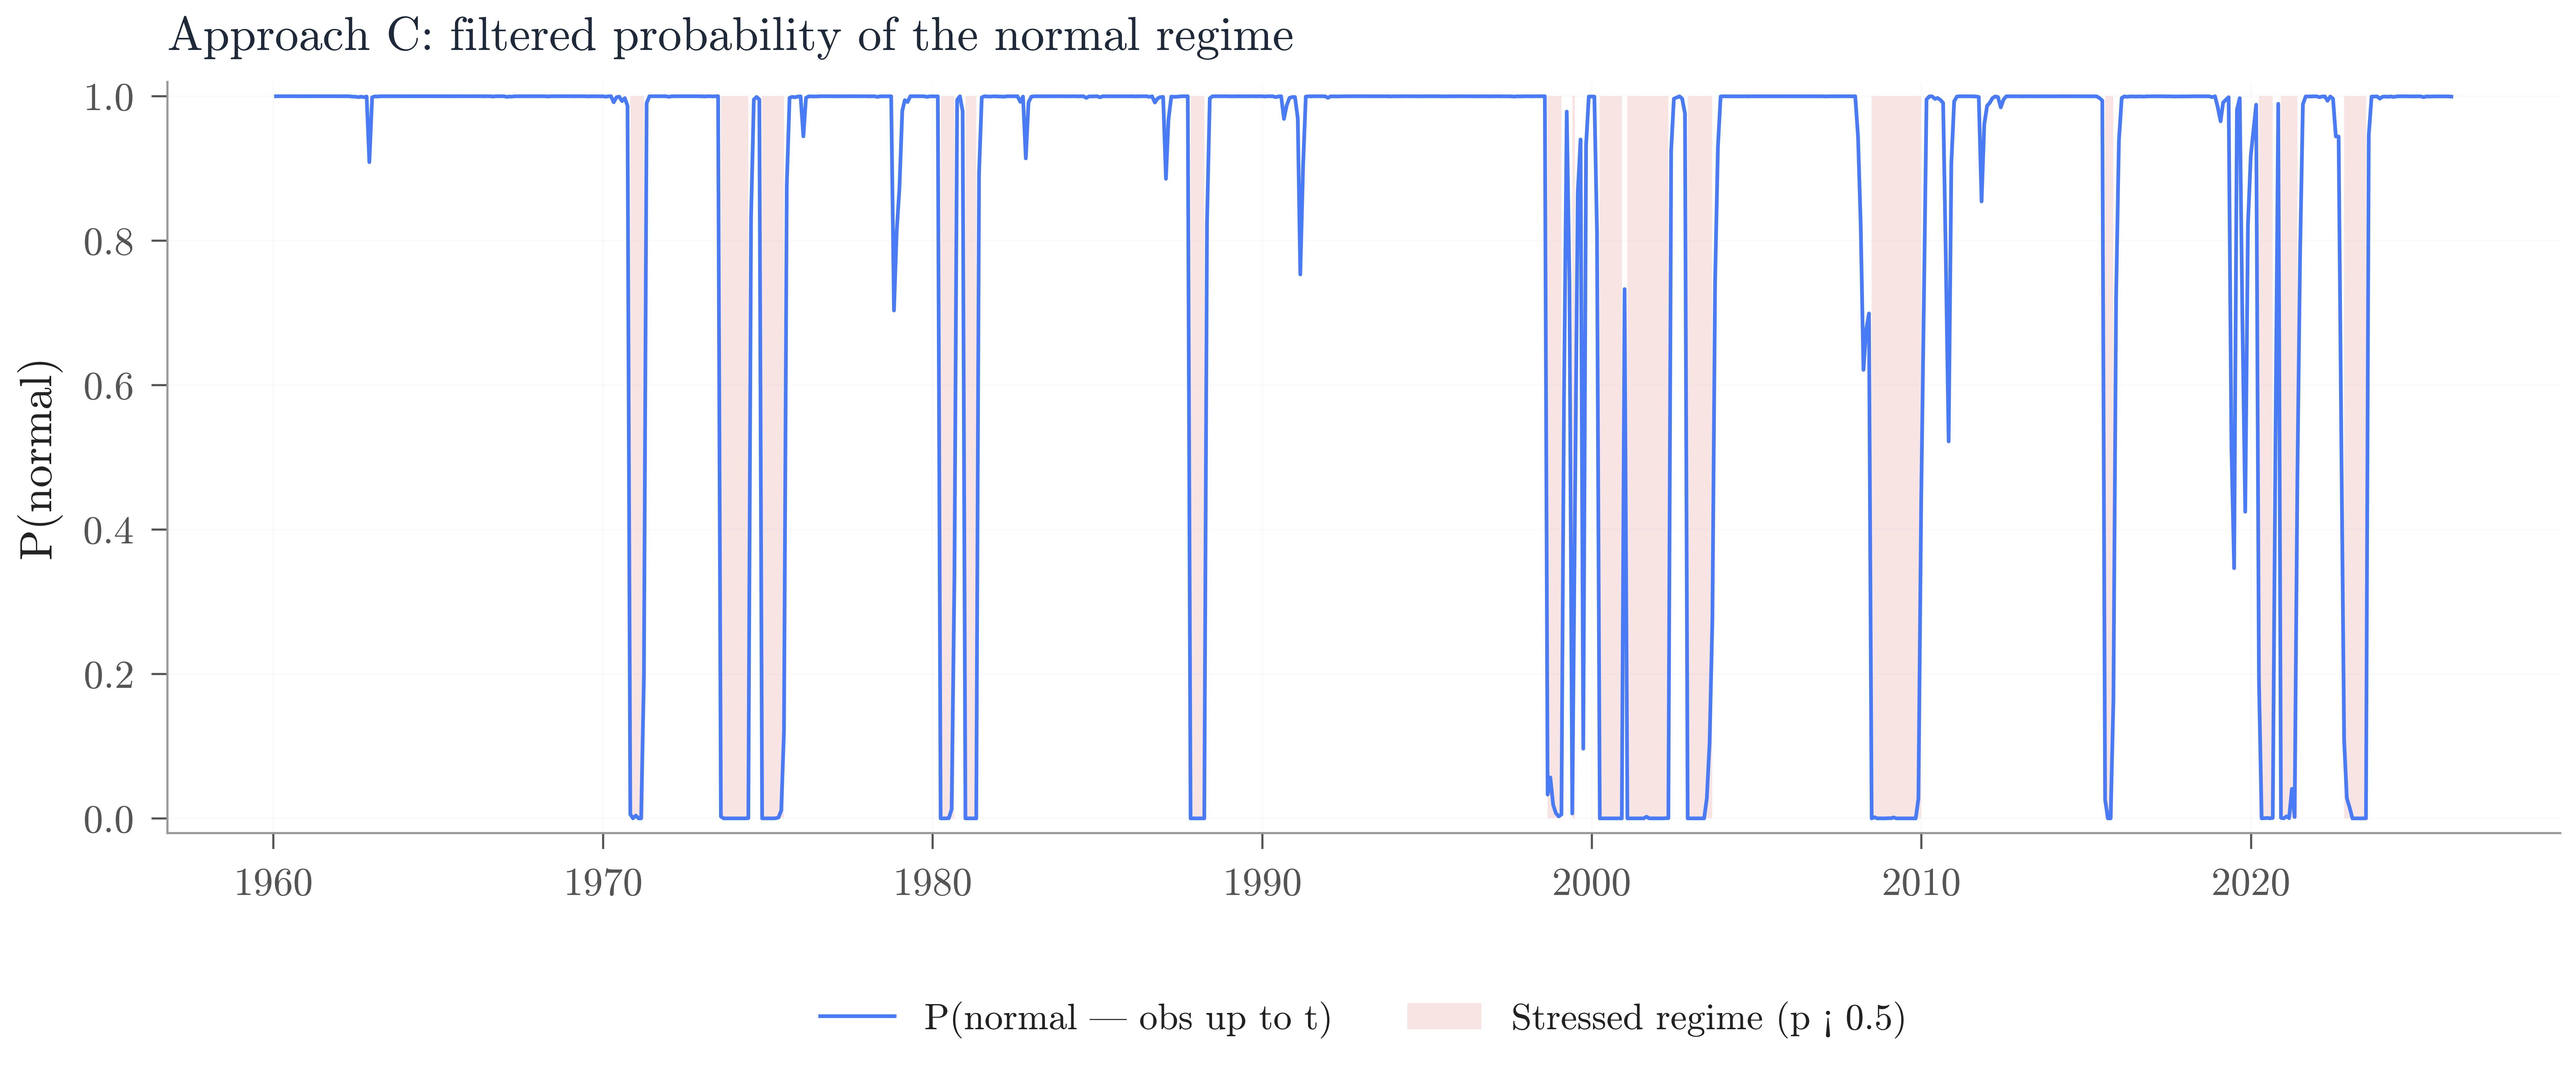
\includegraphics[width=0.85\textwidth]{figures/16_approach_c_pnormal_timeseries.png}
  \end{center}
  \vspace{-2pt}
  \footnotesize Sharpe \textbf{0.72} (CI $[0.46,\,0.96]$), \emphp{essentially ties DM} without any hand-crafted features.
\end{frame}

% =========================================================
% SLIDE 9: THE ENSEMBLE
% =========================================================
\begin{frame}{None alone beats DM. What if we average them?}
  \vspace{8pt}
  \begin{equation*}
    w^{\fundname}_t \;=\; \mathrm{clip}_{[-1,\,+3]}\!\left( 0.5 \cdot w^{DM}_t \;+\; 0.25 \cdot \mathbb{1}\{\hat{p}^{\text{crash}}_t < 0.05\} \;+\; 0.25 \cdot P(\text{normal}_t) \right)
  \end{equation*}
  \vspace{8pt}
  \begin{itemize}
    \item \textbf{Majority weight on DM} (the strongest single linear signal)
    \item Shield (B) and HMM (C) as complementary regime overlays
    \item \textbf{Not fragile}: equal thirds and 0.4/0.3/0.3 also deliver Sharpe \textbf{0.80}
  \end{itemize}
  \vspace{12pt}
  \emphb{Research question:} can the components' error structures really be different enough for averaging to help?
\end{frame}

% =========================================================
% SLIDE 10: EMPIRICAL DECORRELATION
% =========================================================
\begin{frame}{Why the ensemble works: decorrelation evidence}
  \vspace{4pt}
  Pairwise correlation of each component's \textbf{edge over DM} (return minus DM return):
  \vspace{12pt}
  \begin{center}
  \small
  \begin{tabular}{l r r r}
    \toprule
     & \textbf{A (Ridge)} & \textbf{B (Shield)} & \textbf{C (HMM)} \\
    \midrule
    A (Ridge)  & 1.00 & \emphp{0.31} & \emphp{0.28} \\
    B (Shield) & 0.31 & 1.00 & 0.66 \\
    C (HMM)    & 0.28 & 0.66 & 1.00 \\
    \bottomrule
  \end{tabular}
  \end{center}
  \vspace{18pt}
  \begin{itemize}
    \item A's edge is \emphp{nearly uncorrelated} with B and C ($\rho \approx 0.30$)
    \item Averaging cancels noise faster than it cancels signal
    \item Ensemble Sharpe \textbf{0.80} dominates every component: DM 0.74, A 0.69, B 0.63, C 0.72
  \end{itemize}
\end{frame}

\end{document}
